In this chapter, we will focus our attention on Redis. Redis is officially described as ``in-memory data structure store, used as database, cache and message broker.'' \cite{sanfilippo2009redis} Like Memcached, Redis provides a simple text based API with \textit{get}, \textit{set}, and many more advanced features, for interaction over the network. Unlike Memcached, Redis is single threaded by design which introduces interesting scalability challenges.

We initially focus on the default performance of Redis when it is first deployed. Subsequently, we will turn our attention to Redis scalability as well as performance under various scenarios. We will consider the effect of multiple Redis instances, process pinning and IRQ Affinity. Furthermore we will explore Redis performance with different object sizes and key distributions.

Throughout this chapter, we focus on key performance metrics - throughput, mean and tail (99th) percentile latency as well as the target Quality of Service (QoS) of 99th percentile latency within 1 millisecond. Unless otherwise stated, all benchmarks are performed to target the QoS.


\section{Out of the Box Performance}
Firstly, we focus on the default Redis performance. Redis comes with a configuration file \texttt{redis.conf}\cite{RedisConfiguration} with sensible defaults. Redis supports data persistence management and by default keys are not evicted when the cache fills up. For the purposes of this paper, we are interested an eviction based cache and as such will configure Redis to use the Least Recently Used policy for key replacement. Configuration options can be supplied on the command line as well and override any configuration options specified in \texttt{redis.conf}. Table \ref{tab:r_redis_baseline_config} summarizes our default Redis configuration.

\begin{table}[h!]
\centering
\begin{tabular}{| c c c |}
 \hline
 Configuration Option & Explanation & Value\\ [0.5ex]
 \hline\hline

 --port & Port number & 11120 \\
 --maxmemory & Maximum used memory & 6GB \\
 --maxmemory-policy & Policy for key evictions & allkeys-lru \\

 \hline

\end{tabular}
\caption{Redis Configuration}
\label{tab:r_redis_baseline_config}
\end{table}

With the configuration defined, we can deploy the Redis application with the following command.

\begin{lstlisting}
redis redis.conf --port 11120 --maxmemory=6GB
    --maxmemory-policy=allkeys-lru
\end{lstlisting}

In order to get an initial feel for Redis performance, we setup the benchmark to increase load on the cache server linearly. Table \ref{tab:r_memtier_baseline_config} outlines the configuration used for the Memtier benchmark.

\begin{table}[h!]
\centering
\begin{tabular}{| c c c |}
 \hline
 Configuration Option & Explanation & Value\\ [0.5ex]
 \hline\hline

 -s & Server & nsl200 (server hostname) \\
 -p & Port number & 11120 \\
 -c & Number of Connections & [1..10] \\
 -t & Number of Threads & 2 \\
 --key-minimum & Smallest key & 1 \\
 --key-maximum & Largest key & 100 000 000 \\
 --random-data & Generate Random Data & true \\
 --data-size & The size of data in bytes & 64 \\

 \hline

\end{tabular}
\caption{Memtier Configuration Options}
\label{tab:r_memtier_baseline_config}
\end{table}

Memtier can be started with the following command:
\begin{lstlisting}
  memtier -s <server> -p 11120 -c <connections> -t 2
    --random-data
    --key-minimum=1
    --key-maximum=100000000
    --random-data
    --data-size=64
\end{lstlisting}

We are showing the Redis deployment command as well as the Memtier command here for clarity, however, the commands will be omitted in subsequent sections.

\subsection{Latency \& Throughput vs Connections}
\begin{figure}[h]
    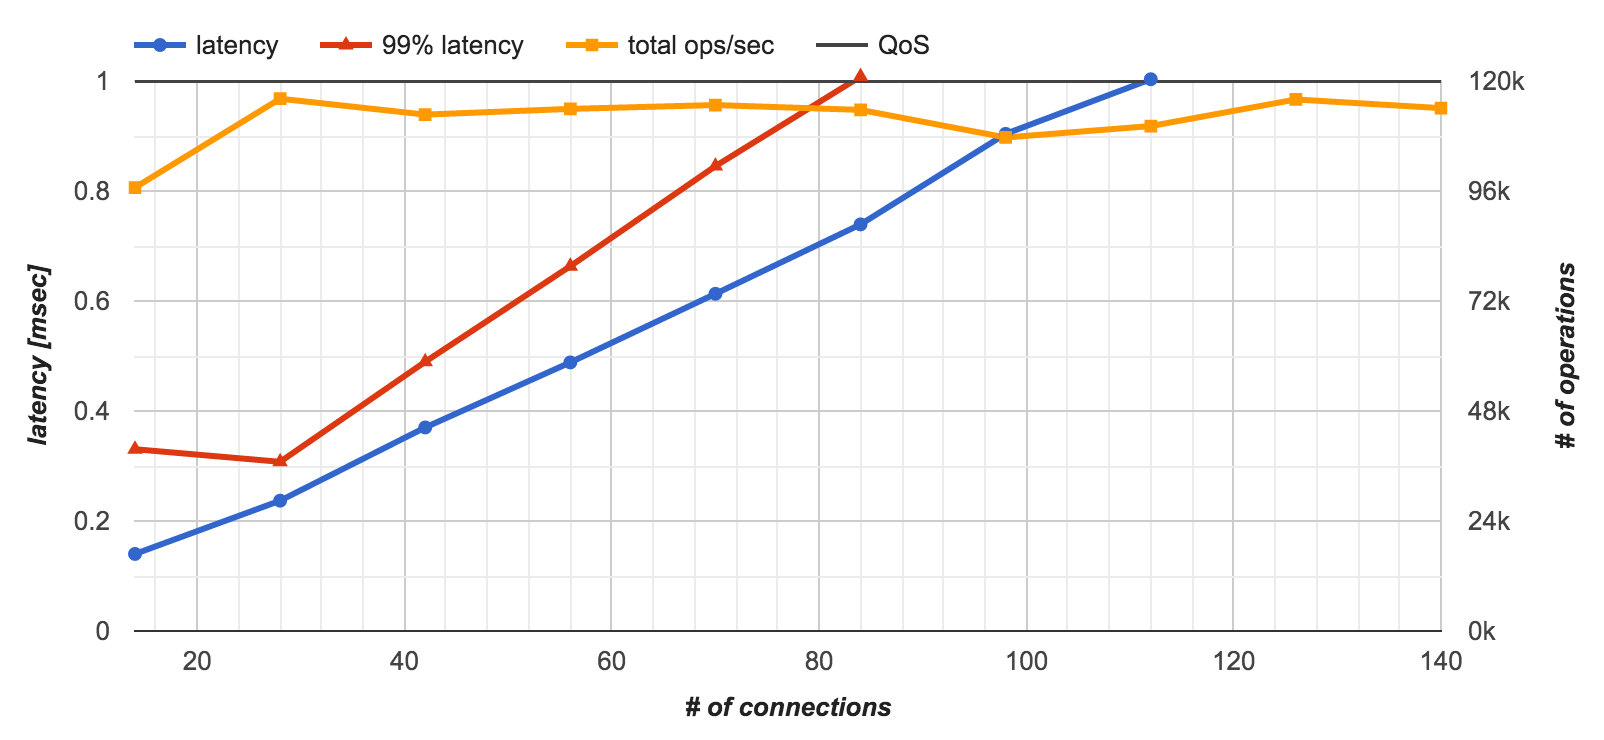
\includegraphics[width=\textwidth]{./res2/r_baseline_latency.png}
    \caption{Latency \& Throughput vs Number of Connections}
    \label{fig:r_baseline_latency}
\end{figure}

Figure \ref{fig:r_baseline_latency} plots the relationship between mean latency, 99th percentile latency and the number of operations per second against the number of connections.
The mean latency increases with the number of connections linearly. Similarly, the 99th percentile latency increases linearly as the number of connections increases, however, it grows faster than the man latency. At 56 connections, we obtain a 99th percentile latency of 0.88 ms. A further increase in the number of connections leads to QoS violation.
The number of operations per second remains constant with the number of connections and latency within QoS. The cache executes 93k requests per second, however, at this load we are unable to increase throughput while satisfying our QoS.

\subsection{CPU Utilization}
\begin{figure}[h]
    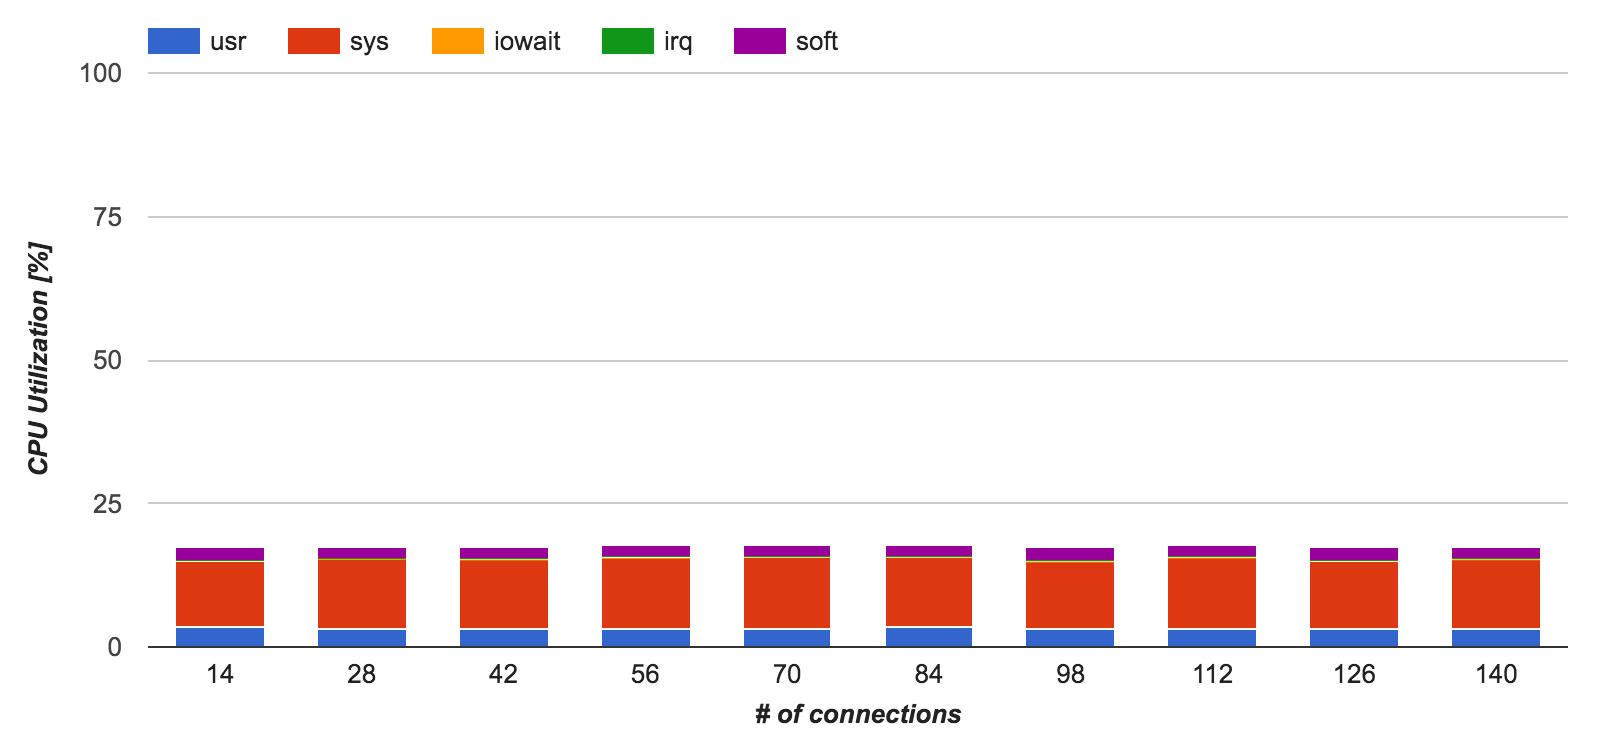
\includegraphics[width=\textwidth]{./res2/r_baseline_cpu.png}
    \caption{Default Redis CPU Utilization vs Number of Connections}
    \label{fig:r_baseline_cpu}
\end{figure}

Figure \ref{fig:r_baseline_cpu} plots the relationship between CPU utilization as reported by \textit{mpstat} and the number of connections. Firstly, we can observe that the total utilization remains stable at 17\%. We can clearly see that overall the server is heavily underutilized. However, the aggregate breakdown across all CPUs is misleading in this case. Figure \ref{fig:r_baseline_cpu_individual} shows the individual CPU utilization for 56 client connections. We can observe that we achieve nearly 100\% utilization on core 0 while the remaining cores are idle. Furthermore, we can observe that Redis accounts for only 14\% utilization while the rest is used for kernel processing (46\%) and software interrupt processing (34\%). From the breakdown, we can conclude Redis utilization is kernel and software interrupt dominated rather than application processing dominated.

\begin{figure}[h]
    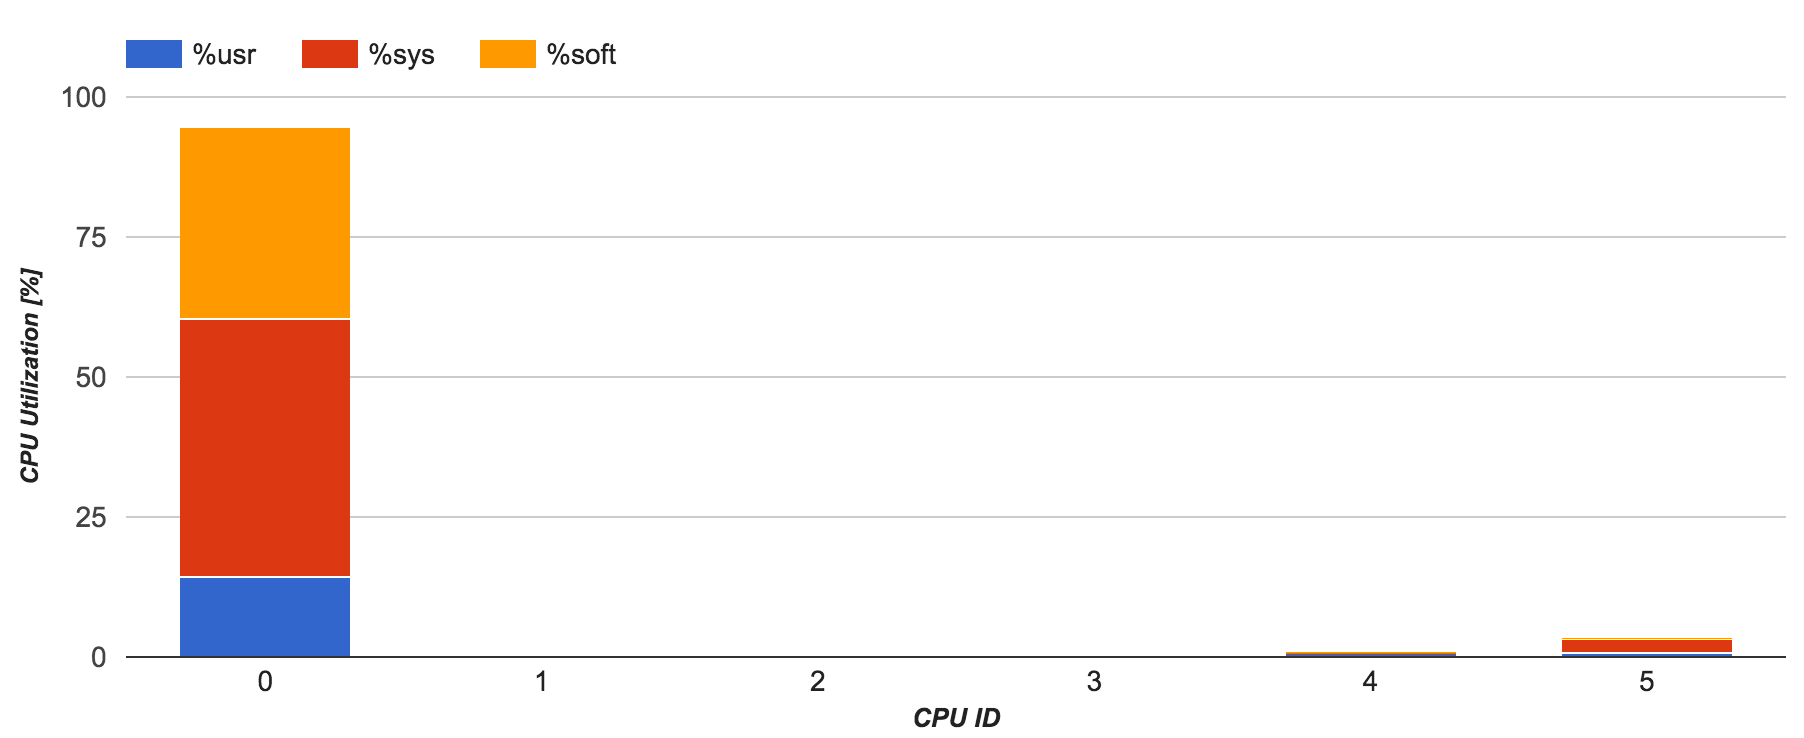
\includegraphics[width=\textwidth]{./res2/r_baseline_cpu_individual.png}
    \caption{Default Redis Individual CPU Utilization at 56 connections}
    \label{fig:r_baseline_cpu_individual}
\end{figure}

\subsection{Conclusion}
We have shown that Redis is capable of delivering 93k requests per second in its default configuration without any optimizations. Additionally, we have observed the impact of single threaded Redis on the overall host CPU utilization as well as the breakdown per individual core. We have also shown that the kernel and software interrupt processing play a significant role in overall performance.


\section{Multiple Redis Instances}
\label{sec:multiple-redis-instances}

As seen in previous section, the overall cache server utilization suffers from single threaded nature of Redis. An immediate solution to this problem is to deploy multiple instances simultaneously. In this section, we consider a multi-instance Redis setup. It is important to keep in mind that each individual instance is completely isolated from the rest. As a result, the amount of memory space available to each instance decreases and therefore the key range we can store on each instance decreases. An application requiring access to a large number of keys will therefore be forced to partition the key space. Client side consistent hashing has the ability to alleviate this problem. Alternatively, a proxy application such as Twemproxy \cite{twemproxy} can be used to spread the load and create a single point of access to the instances.

As the number of instances increases on the server, we expect the overall throughput to increase. As such, we initially utilize a larger number of connections than in the previous section, namely we use 210 connections (30 connections per each benchmarking host). We have determined empirically that 30 connections allow us to demonstrate Redis multi-instance scalability effectively. Additionally, 30 provides a great deal of flexibility when dealing with load partitioning across instances as we have 6 CPU cores available to us on the server. We consider 5 distinct multi-instance scenarios, they breakdown is outlined in Table \ref{tab:redis_instances}.

\begin{table}[h!]
\centering
\begin{tabular}{| c c c c |}
 \hline
 Instance Count & Connections & Threads & Total\\ [0.5ex]
 \hline\hline

 1  & 5 & 6 & 30 \\
 2  & 5 & 3 & 30 \\
 3  & 5 & 2 & 30 \\
 6  & 5 & 1 & 30 \\
 10 & 3 & 1 & 30 \\
 \hline

\end{tabular}
\caption{Multi Instance Scenarios with Memtier connections and thread counts}
\label{tab:redis_instances}
\end{table}

Consequently, we can define the following Redis configuration for each scenario. We maintain the same amount total memory while partitioning it evenly across instances. We of course also use the LRU Redis policy.

\begin{table}[h!]
\centering
\begin{tabular}{| c c c |}
 \hline
 Instances & Memory & Total Memory\\ [0.5ex]
 \hline\hline

 1  & 6GB & 6GB \\
 2  & 3GB & 6GB \\
 3  & 2GB & 6GB \\
 6  &  1GB & 6GB \\
 10 &  0.6GB & 6GB \\
 \hline

\end{tabular}
\caption{Redis Maximum Memory config per number of instances}
\label{tab:redis_instances}
\end{table}


\subsection{Latency \& Throughput vs Instances}
\begin{figure}[h]
    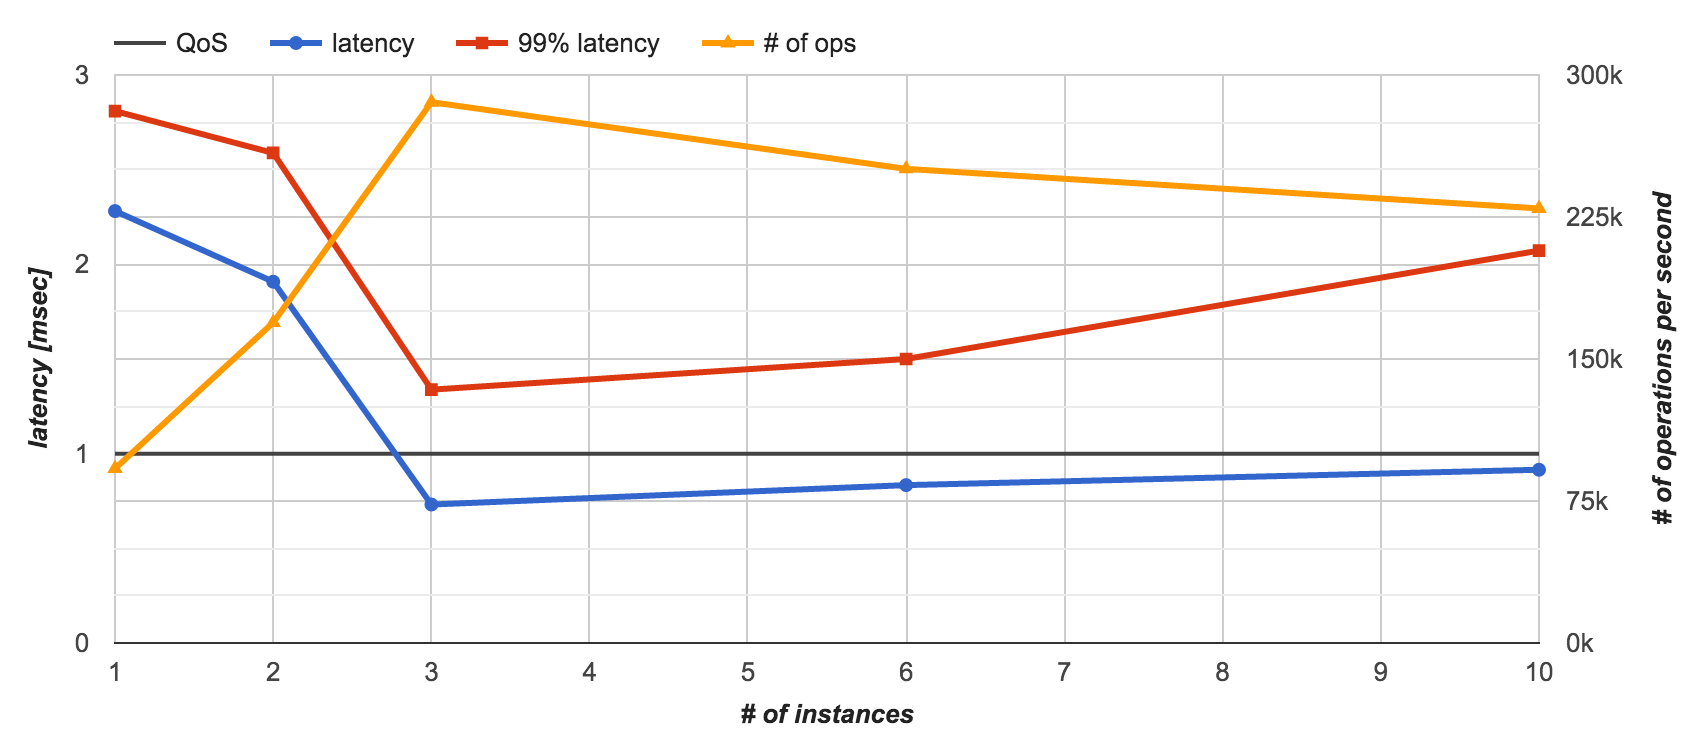
\includegraphics[width=\textwidth]{./res2/r_instances_latency.png}
    \caption{Redis Instances: Latency \& Throughput}
    \label{fig:r_instances_latency}
\end{figure}

Figure \ref{fig:r_instances_latency} plots the relationship between latency, throughput and the number of instances.

Firstly, as the number of instances increases, both 99th and mean latency decrease and a reach a minimum at 3 instances. At 3 instances, we obtain a 99th percentile latency of 1.33 milliseconds, above the requires QoS. As the number of instances increases further, both mean and tail latency increase too.

Secondly, as the number of instances increases, throughput does too up to 3 instances where it reaches a maximum of 285k requests per second. A further increase in the number of instances leads to a decrease in throughput.

We can observe that multiple Redis instances do not scale as expected. We would expect the maximum throughput with the minimum tail latency to be achieved at 6 instances as we have 6 cpu cores. However, we maximize throughput while minimizing tail latency at 3 instances instead. Let us investigate the CPU utilization to get a better insight into the problem.

\subsection{CPU vs Instances}
\begin{figure}[h]
    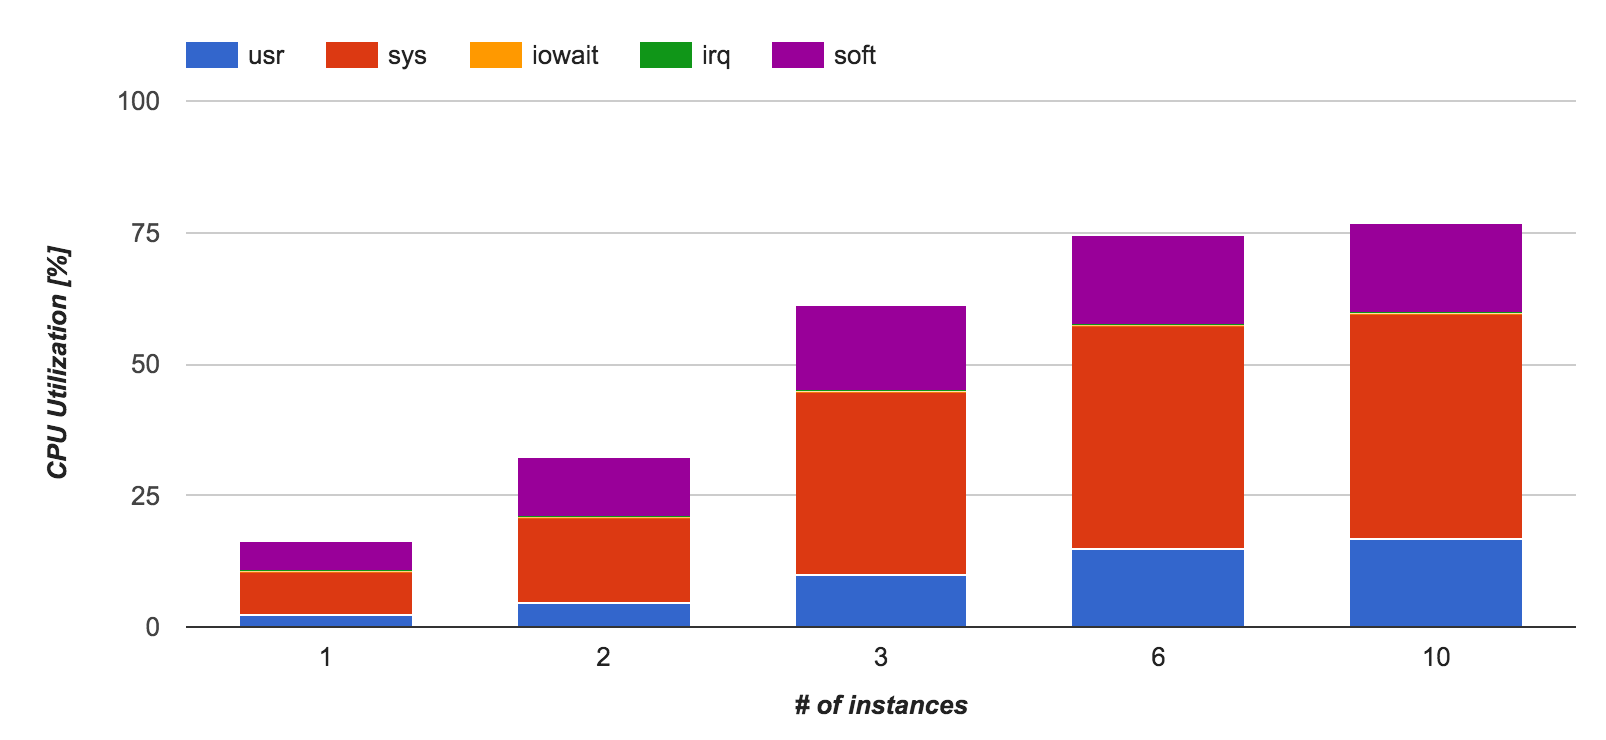
\includegraphics[width=\textwidth]{./res2/r_instances_cpu.png}
    \caption{Redis Instances CPU}
    \label{fig:r_instances_cpu}
\end{figure}

Figure \ref{fig:r_instances_cpu} plots the CPU utilization against the number of instances with the respective category breakdown as reported by \textit{mpstat}. We can observe that as we increase the number of instances, total CPU utilization increases. However, at no point do we reach a 100\% utilization on the server. The utilization remains capped at 75\% for configurations with 6 and 10 instances. Let us investigate the distribution of work on individual cores to get a better insight into the problem.

Figure \ref{fig:r_instances_cpu_individual} outlines the CPU utilization per individual CPU core with 6 instances. We can observe that all software interrupts are processed on core 0 with 100\% utilization while the remaining cores remain underutilized. This renders core 0 a bottleneck for the remaining CPU cores and results in underutilization of resources.

\begin{figure}[h]
    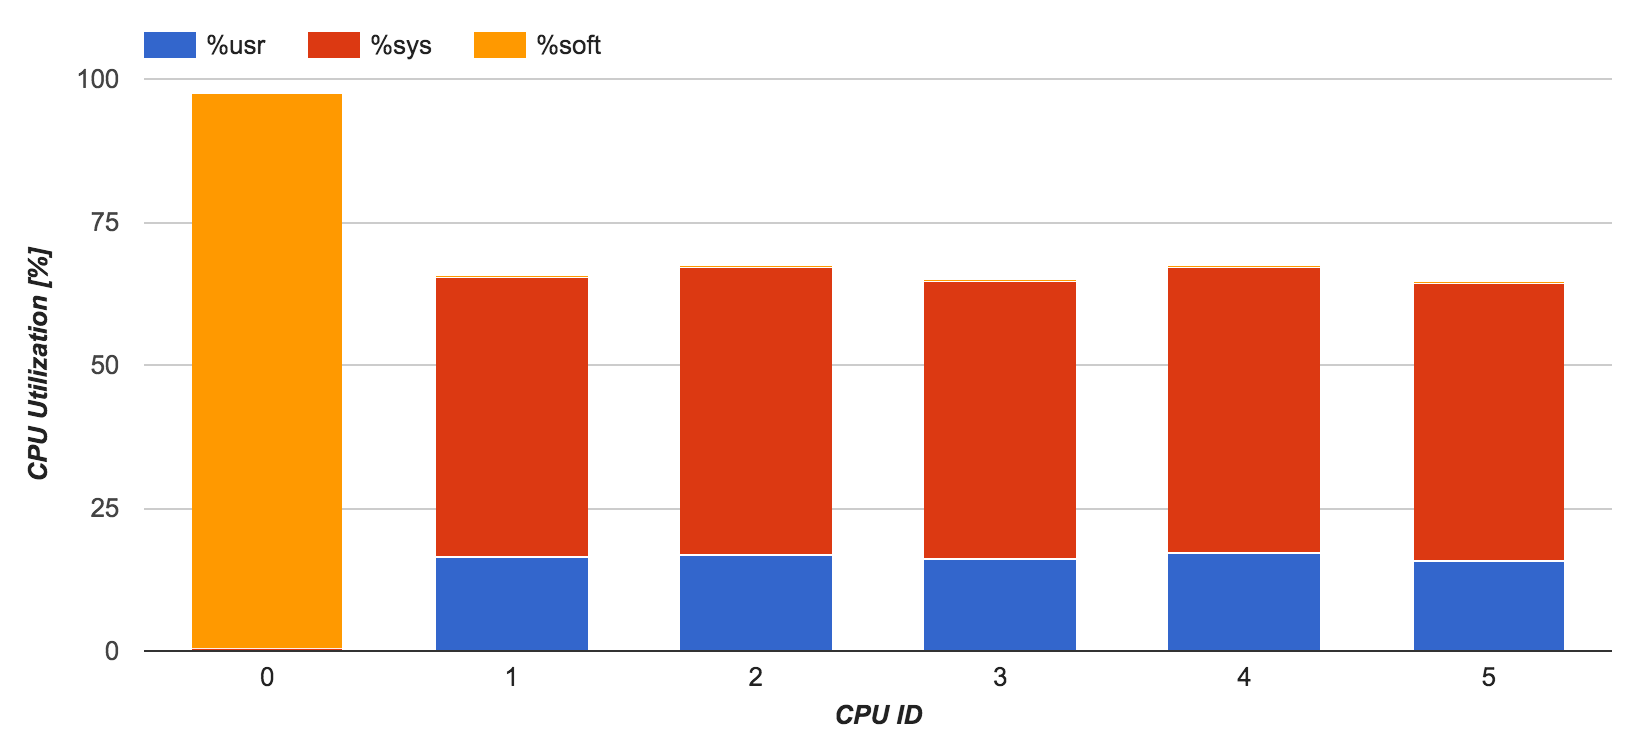
\includegraphics[width=\textwidth]{./res2/r_instances_cpu_individual.png}
    \caption{Redis Instances: Individual CPU Utilization at 6 instances}
    \label{fig:r_instances_cpu_individual}
\end{figure}

\subsection{Multiple Instances Conclusion}
We have shown that multiple Redis instances do not scale linearly with the number of instances. In our benchmark, we have observed that the software interrupt processing is the bottleneck of multiple instances. We will address the load imbalance problem in the following chapter through IRQ Affinity pinning.

% ____________________________________________________
\section{IRQ Affinity}
In this chapter we turn our attention to addressing the load imbalance problem observed in when scaling Redis across multiple instances. In order to spread the software interrupt processing work across to multiple cores, we will assign each individual core a unique CPU core affinity. This process is outlined in detail in Section \ref{sec:m_irq_affinity}.

With IRQ Affinity assigned, we would expect the software interrupt processing to be spread evenly across all CPU cores and therefore removing the single CPU core bottleneck observed in the previous chapter.

\subsection{Latency \& Throughput with IRQ Affinity}
\begin{figure}[h]
    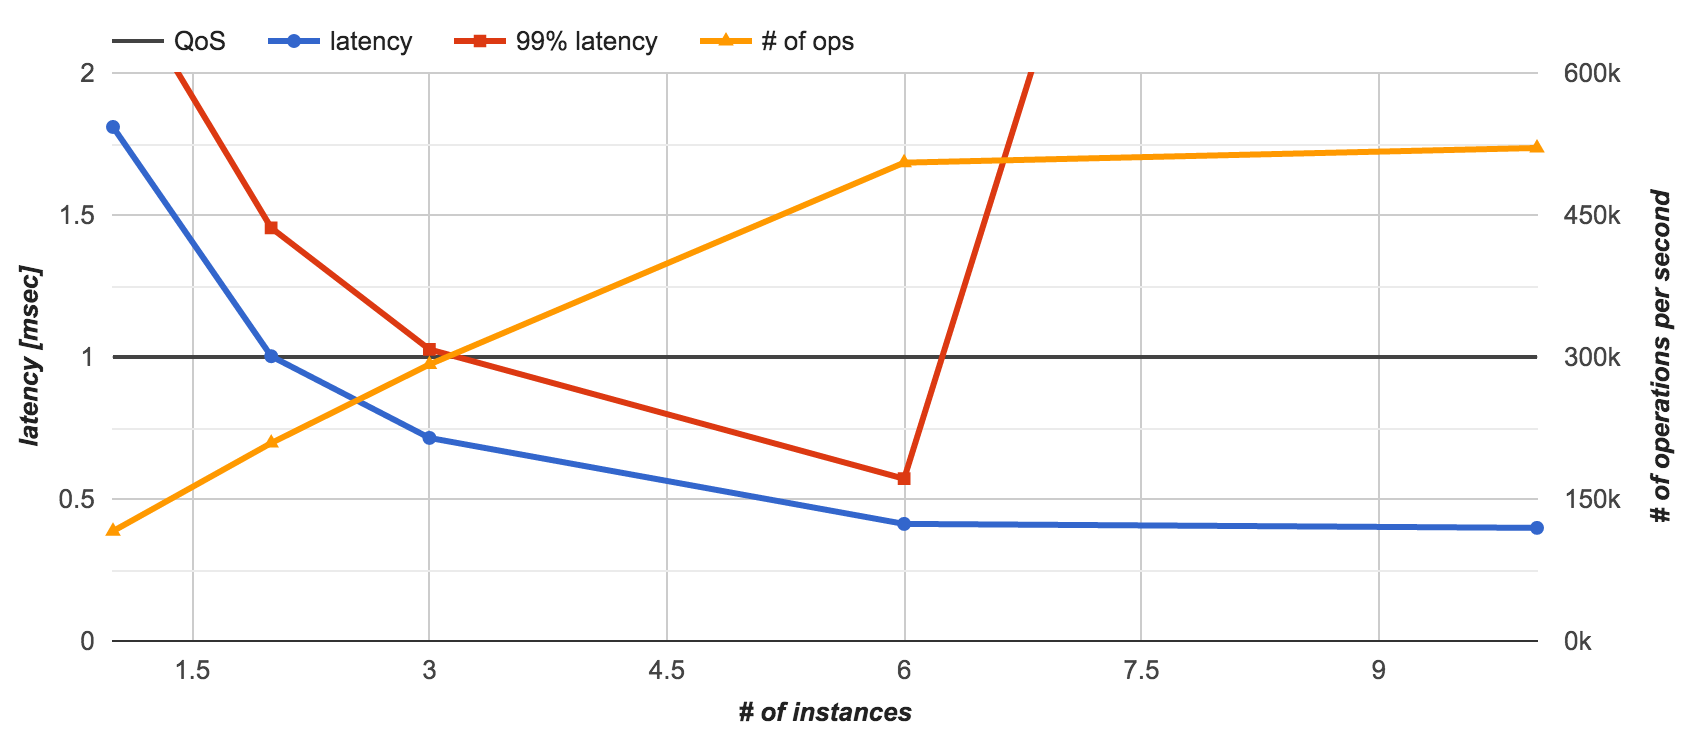
\includegraphics[width=\textwidth]{./res2/r_irq_latency.png}
    \caption{Redis Instances with IRQ Pinned: Latency \& Throughput}
    \label{fig:r_irq_latency}
\end{figure}

\subsection{CPU Utilization with IRQ Affinity}
\begin{figure}[h]
    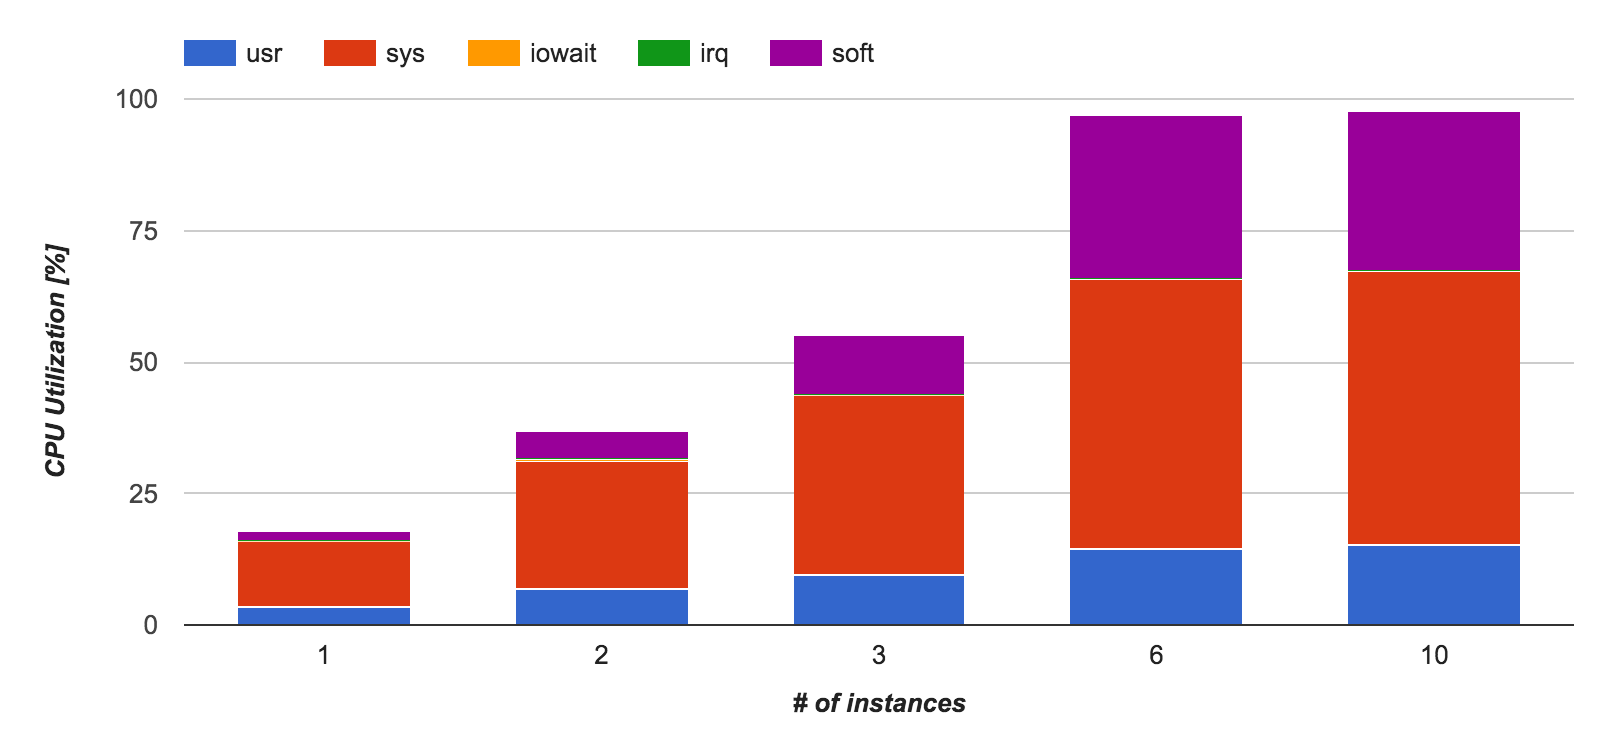
\includegraphics[width=\textwidth]{./res2/r_irq_cpu.png}
    \caption{Redis Instances with IRQ Pinned: CPU Utilization}
    \label{fig:r_irq_cpu}
\end{figure}
\begin{figure}[h]
    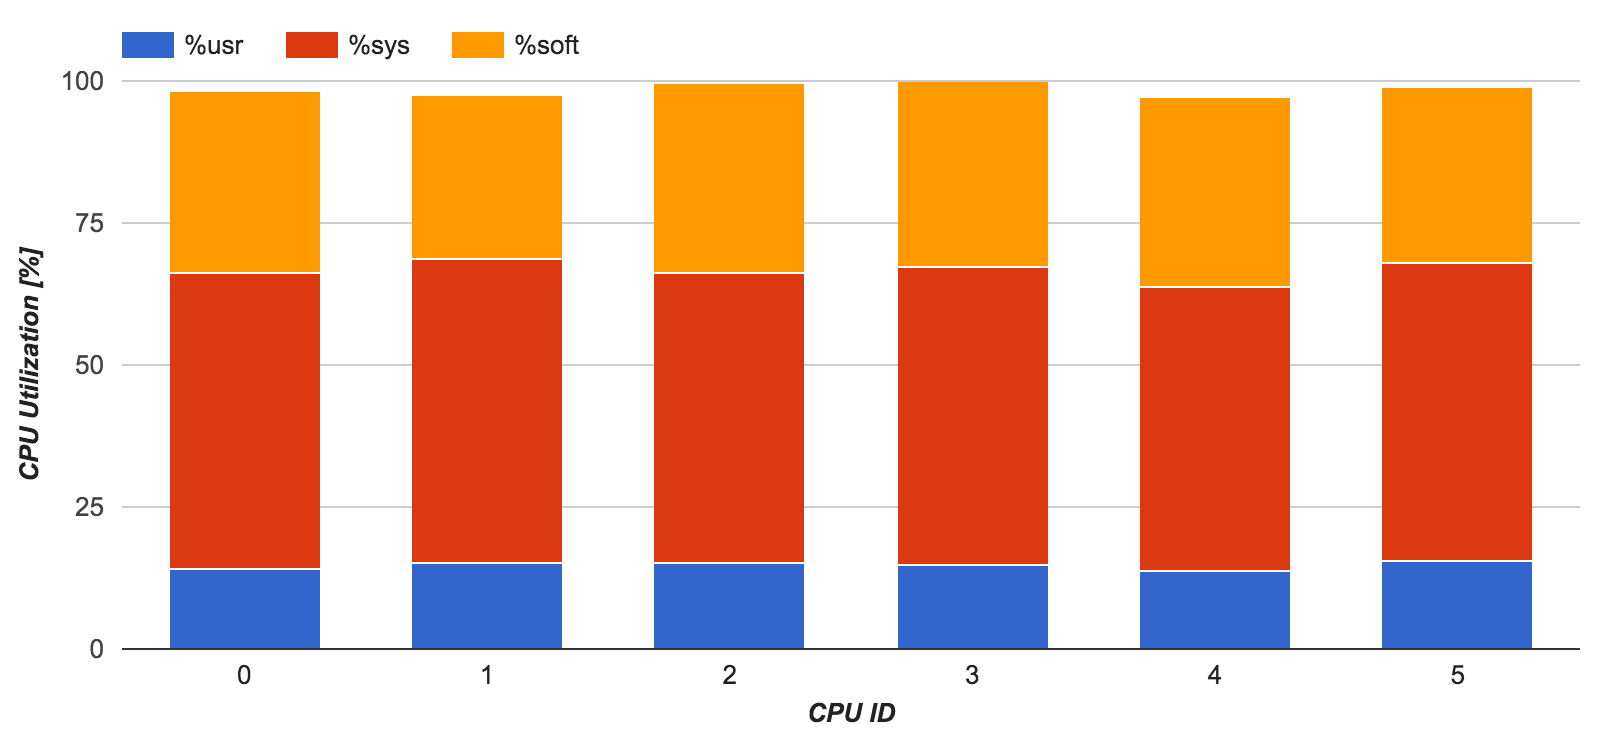
\includegraphics[width=\textwidth]{./res2/r_irq_cpu_individual.png}
    \caption{Redis Instances with IRQ Pinned: Individual CPU utilization at 6 instances}
    \label{fig:r_irq_cpu_individual}
\end{figure}

% % ____________________________________________________

% \section{Pinned Redis Instances}

% In the previous section we have observed that the performance of a Redis server can be greatly improved by provisioning multiple Redis instances simultaneously. Pinning processes to distinct cores is suggested to improve tail latency \cite{leverich2014reconciling}. In this section, we examine the effect process pinning has on the performance of Redis. We consider exactly the same workload as in the previous section \ref{sec:multiple-redis-instances} as well as exactly the same server setup with the exception of pinning the Redis processes. That is, the workload is kept constant while it is partitioned across multiple instances.

% A Redis process can be pinned to a unique core through the use of the \texttt{taskset} utility as follows:

% \begin{lstlisting}
% taskset -pc <redis_pid> <core_id>
% \end{lstlisting}

% The Redis processes identified as \texttt{redis pid} is pinned to the CPU core identified by \texttt{core id}. We can identify the process id of a Redis application through the \texttt{ps} command. When running more Redis applications than there are CPUs, we assign it to the \textit{n}th index of the application modulo the total number of cores, which is 6.


% \subsection{Pinned Latency and Throughput}

% \begin{figure}[h]
%     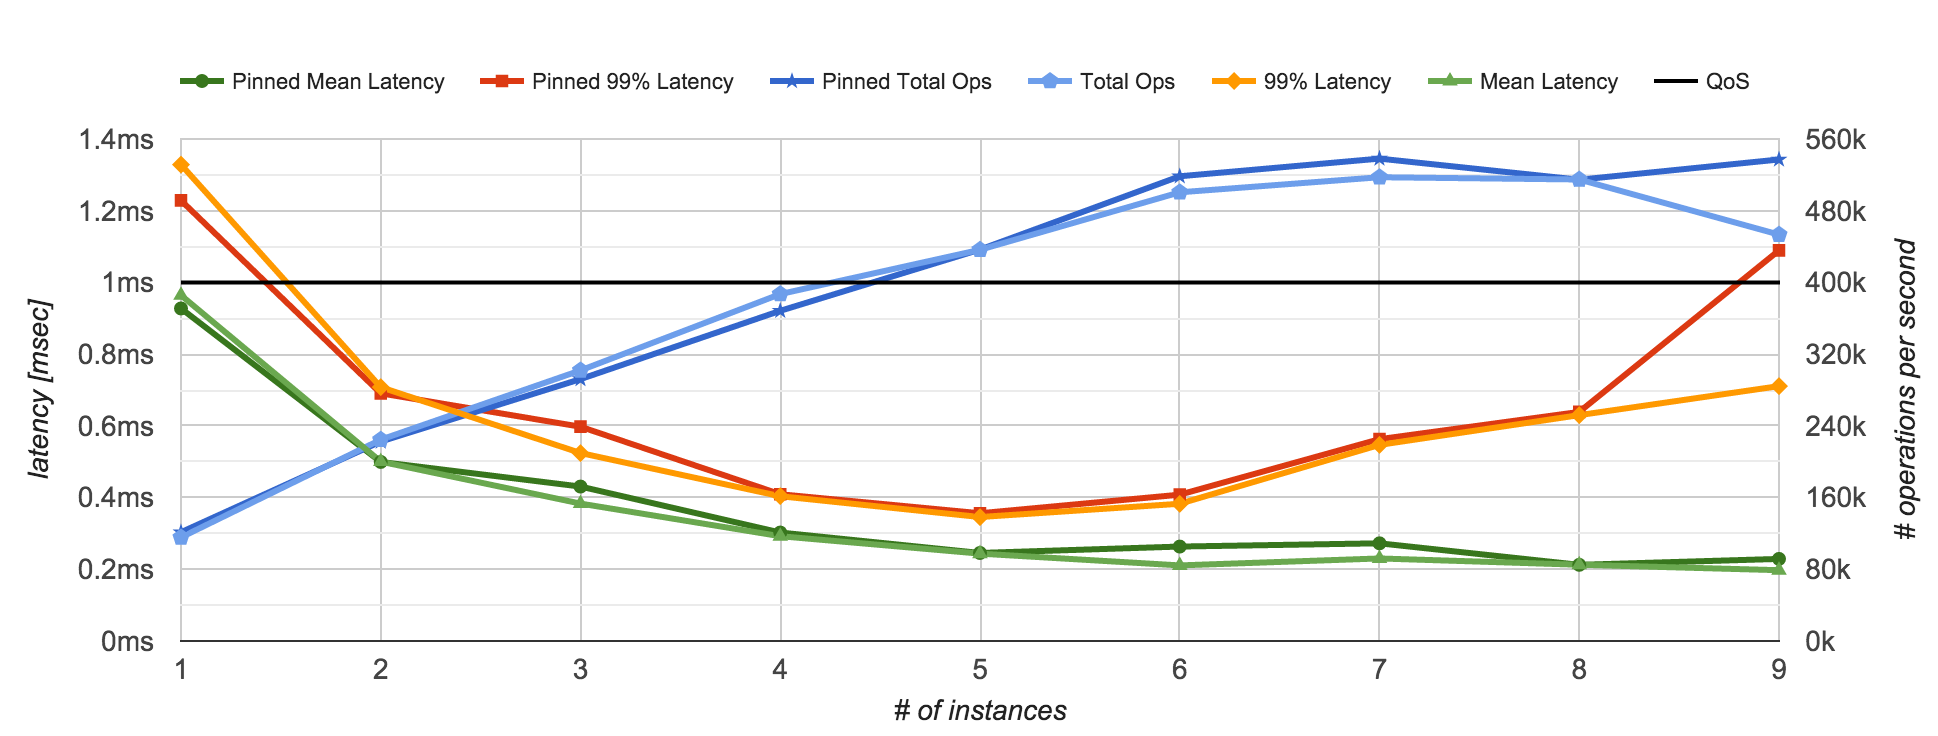
\includegraphics[width=\textwidth]{./res/6_pinned.png}
%     \caption{Redis Instance Pinning: Instances vs Latency and Throughput}
%     \label{fig:6_pinned.png}
% \end{figure}

% Figure \ref{fig:6_pinned.png} plots the relationship between the number of instances on the horizontal axis, latency on the left vertical and throughput on the right vertical. Additionally, the performance obtained without pinning are plotted alongside the pinned results.

% We can observe that pinning  Redis processes results which strongly correlate to the results of the unpinned benchmark. Across mean latency, 99th percentile latency and throughput, there is very little variance in the performance observed.


% \subsection{Redis Persistence}
% TODO


% \section{Object Size}
% In this section, the impact of the size of the object stored in the cache is investigated. Redis imposes no restrictions on the size of objects stored in the cache.

% In order to investigate the impact of object size on the cache, we consider a benchmark with an increasing object size. The object size is increased in powers of two starting at 2 bytes and ranging to 512 KB. This allows us to capture the majority of important sizes commonly used when designing applications.

% The server configuration remains the same as the current best found configuration, the multi-instance configuration with 6 instances. The clients are configured as follows:

% \begin{lstlisting}
% for i in [1..19]
%     memtier -s nsl200 -p <port>
%         -c 3
%         -t 1
%         -P redis
%         --random-data --data-size=pow(2, i)
%         --key-minimum=1 --key-maximum=(1066666666 / pow(2, i))
%         --test-time=400
% \end{lstlisting}

% We run 19 iterations of the benchmark since 512 KB is equivalent to 2 to the power of 19 bytes. The \texttt{data-size} is configured to be increasing in powers of 2. The key range is defined as 6.4 GB split across 6 instances and further accounts for the increased size. Table \ref{tab:6:object_size_latency} outlines the configuration options for each iteration.

% \begin{table}[h!]
% \centering
%  \begin{tabular}{| c || c c c |}
%  \hline
%  Iteration & Data Size (bytes) & Key Maximum & Total Size (GB) \\ [0.5ex]
%  \hline\hline
%     1 & 2 & 53333333 & 6.4 \\ \hline
%     2 & 4 & 26666667 & 6.4 \\ \hline
%     3 & 8 & 13333334 & 6.4 \\ \hline
%     4 & 16 & 6666667 & 6.4 \\ \hline
%     5 & 32 & 3333334 & 6.4 \\ \hline
%     6 & 64 & 1666667 & 6.4 \\ \hline
%     7 & 128 & 833334 & 6.4 \\ \hline
%     8 & 256 & 416667 & 6.4 \\ \hline
%     9 & 512 & 208334 & 6.4 \\ \hline
%     10 & 1024 & 104167 & 6.4 \\ \hline
%     11 & 2048 & 52084 & 6.4 \\ \hline
%     12 & 4096 & 26042 & 6.4 \\ \hline
%     13 & 8192 & 13021 & 6.4 \\ \hline
%     14 & 16384 & 6511 & 6.4 \\ \hline
%     15 & 32768 & 3256 & 6.4 \\ \hline
%     16 & 65536 & 1628 & 6.4 \\ \hline
%     17 & 131072 & 814 & 6.4 \\ \hline
%     18 & 262144 & 407 & 6.4 \\ \hline
%     19 & 524288 & 204 & 6.4 \\ \hline
% \end{tabular}
% \caption{Redis Object Size - Data Size and Maximum Key for each iteration. Total size is calculated as the product of \texttt{Data Size}, \texttt{Key Maximum} and \texttt{6} instances.}
% \label{tab:6:object_size_latency}
% \end{table}


% \subsection{Latency and Throughput}

% \begin{figure}[h]
%     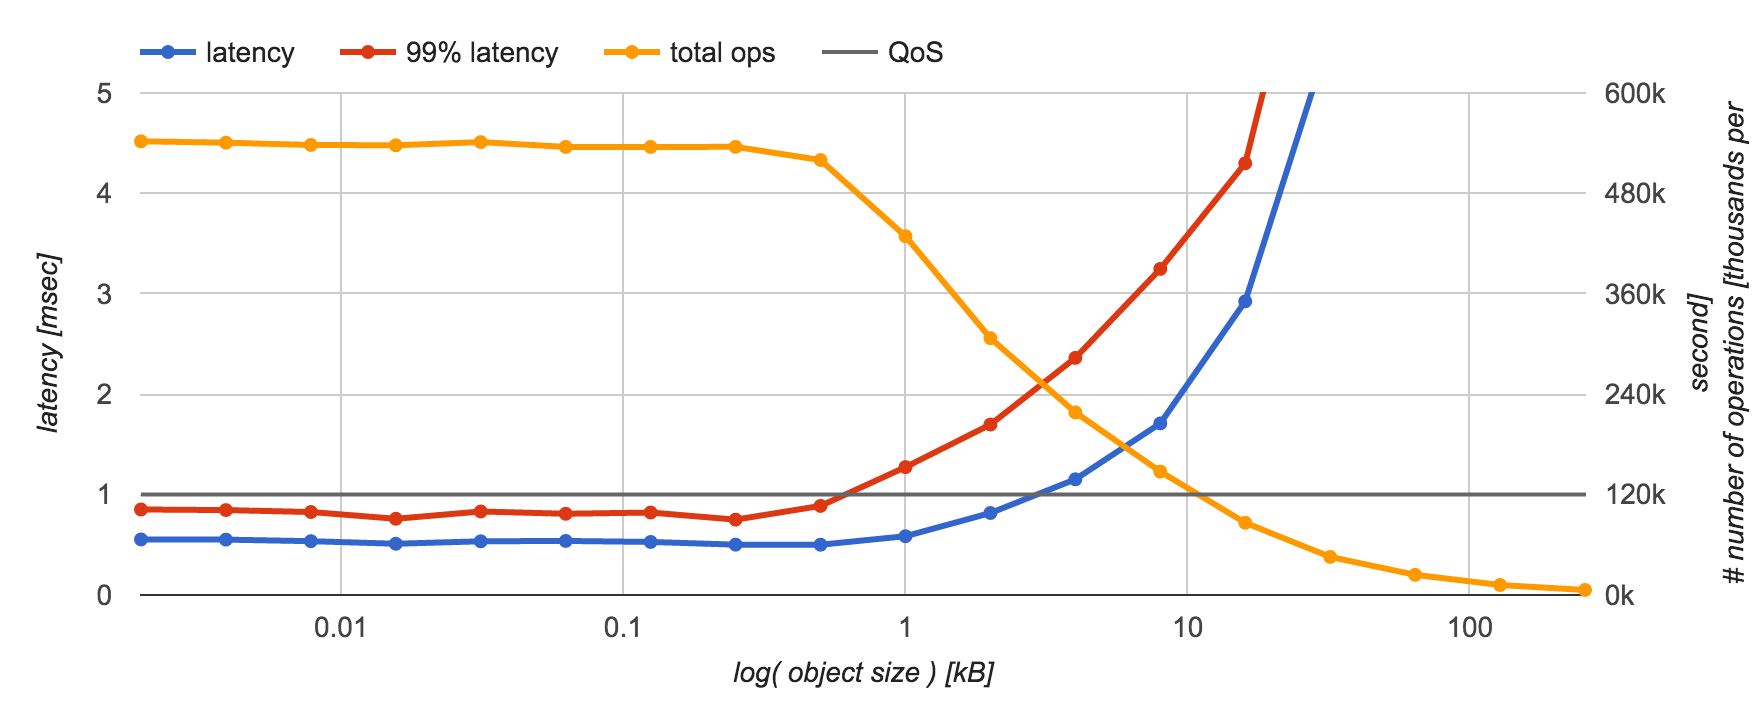
\includegraphics[width=\textwidth]{./res/6_object_size_latency_ops.png}
%     \caption{Redis Object Size: Latency and Throughput}
%     \label{fig:6_object_size_latency_ops.png}
% \end{figure}

% Figure \ref{fig:6_object_size_latency_ops.png} displays the relationship between object size on the horizontal logarithmic axis, latency on the left vertical axis and throughput on the right vertical axis.

% Firstly, as object size increases up to 512 bytes, the mean latency remains stable at 0.55 ms. Beyond 512 bytes, the mean latency starts to increase and climbs beyond the desired QoS constraint at object size of 4 KB. A further increase in object size leads an disproportionately greater increase in mean latency.

% Secondly, the 99th percentile follows the same pattern as the mean latency, however, it begins to climb over the desired QoS sooner, at object size of 1 KB.

% Thirdly, the number of operations per second remains constant for object sizes under 256 bytes. An increase in object size decreases the number of operations per second. This is a reasonable result as an increase in the object size leads to higher bandwidth requirements and therefore leads to a lower number of operations per second.

% Overall, Redis appears to be capable to scale well with object sizes up to 512 bytes. Larger object sizes put additional strain on the cache and require buffering which leads to increased latency of the average, and therefore 99th percentile, request. Primarily, Redis is not designed to store large (1KB+) values. It is, however, possible to partition large values into smaller ones and perform assembly/disassembly of the value on the client side.

% \subsection{CPU Utilization}
% \begin{figure}[h]
%     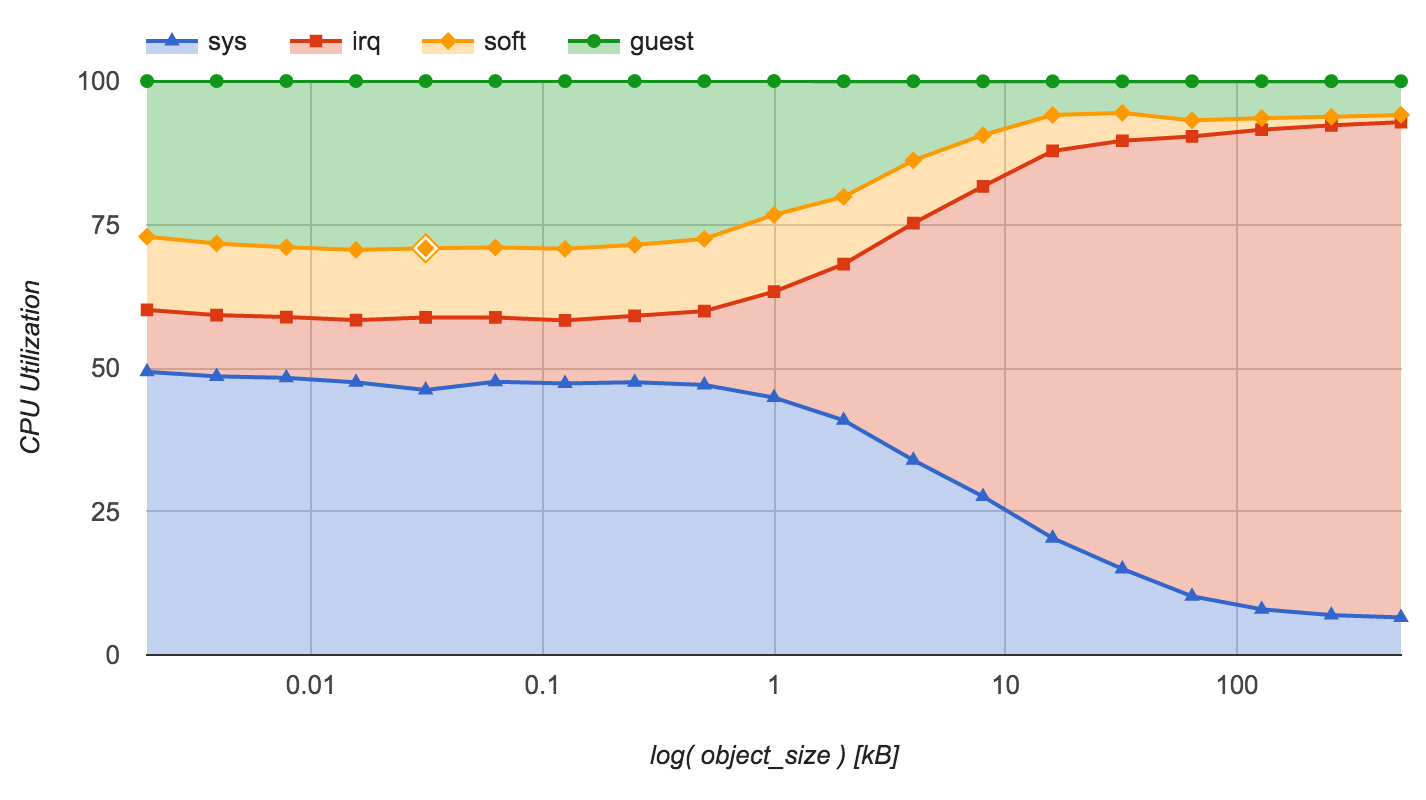
\includegraphics[width=\textwidth]{./res/6_object_size_cpu.png}
%     \caption{Redis Object Size: CPU Usage}
%     \label{fig:6_object_size_cpu.png}
% \end{figure}

% Figure \ref{fig:6_object_size_cpu.png} displays the relationship between object size and CPU usage on the Redis server.

% Firstly, as object size increases up to 1 KB, the operating system (sys) requires about 47 percent of the total time to process the incoming requests and dispatch them to the relevant applications. As object size increases further, the time required decreases as the number of operations decreases.

% Secondly, the Redis applications (guest) require 27 percent of the total time when processing requests under 1 KB, with requests larger the direct cost of running Redis decreases as there are less requests to process. A similar pattern holds for the software interrupts (soft), as there are less requests coming.

% Finally, the time allocated to servicing hardware interrupts (irq) remains at 12 percent below 1KB, with object size increases beyond 1 KB, there is significant increase in the time required to service hardware interrupts. This is due to buffering of large objects and is effectively the cause of high mean and 99th percentile latency as well as low throughput.


% Overall, Redis is designed to work well with objects sizes below 1 KB. As the object size increases, the cache experiences a degraded performance due to buffering of network input and output.

% \section{Key Distributions}
% TODO

% \subsection{Gaussian distribution}
% TODO

% \subsection{Zipf distribution}
% TODO